\subsubsection{SAM with Single infused token}
This section evaluates SAM using a single token prompt strategy. As shown in 
Table \ref{tab:single_token_params}, vit\_b achieves a peak IoU of 0.3771 for 
ARs, while vit\_l performs better on TCs at 0.5694. However, the larger capacity 
of vit\_l introduces significant computational overhead. With 321.74M total 
parameters, it requires approximately 3.23 hours for training compared to the 
2.05 hours needed for the smaller vit\_b architecture.

\begin{table}[h]
\centering
\begin{tabular}{lcccccccc}
\hline
Backbone & IoU AR & IoU TC & Decoder & Encoder & Train & Frozen & Total & \% Train \\
\hline
vit\_l & 0.3015 & 0.5694 & 1.47M & 7.92M & 9.39M & 312.35M & 321.74M & 2.92\% \\
vit\_b & 0.3771 & 0.5292 & 1.07M & 1.58M & 2.65M & 93.74M & 96.40M & 2.75\% \\
\hline
\end{tabular}
\caption{Detailed Parameter Breakdown and Performance for Single Token SAM}
\label{tab:single_token_params}
\end{table}


Training dynamics in Figure \ref{fig:iou_single_token} reveal that the model cannot 
improve ARs and TCs scores at the same time. This inverse relationship 
indicates catastrophic forgetting, where optimization for large scale ARs 
effectively overwrites representations required for localized TCs. The 
single token approach fails to maintain a stable balance across both 
phenomena due to task interference during LoRA adaptation.

\begin{figure}[!h]
    \centering
    \begin{minipage}[b]{0.45\textwidth}
        \centering
        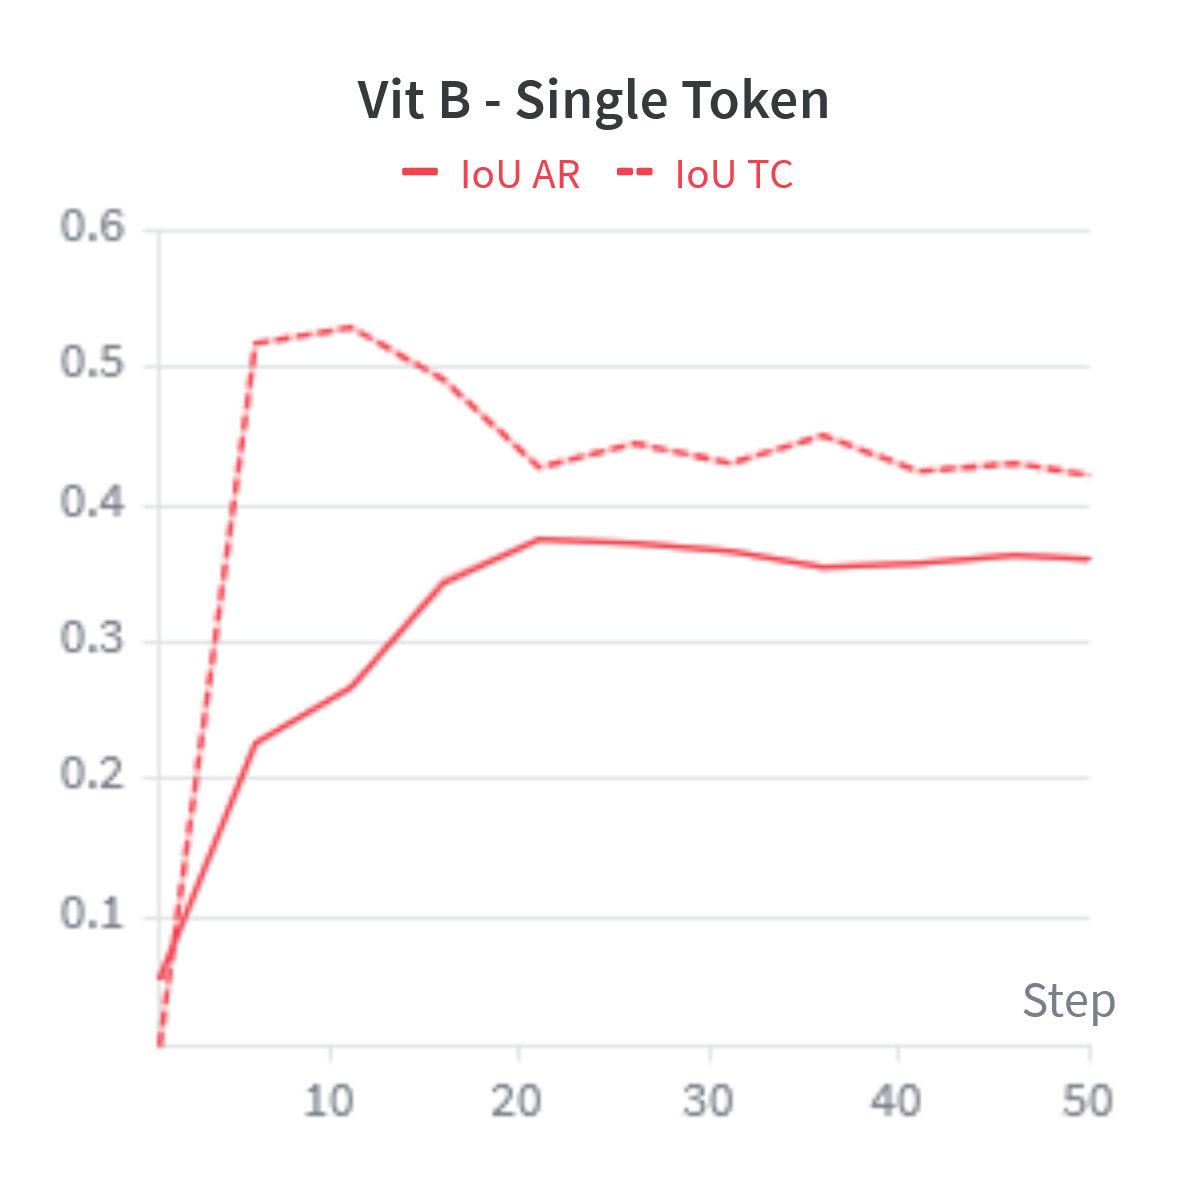
\includegraphics[width=\textwidth]{graphics/result/vitbsingletoken.png}
        % \caption{Vit B}
    \end{minipage}
    \hfill
    \begin{minipage}[b]{0.45\textwidth}
        \centering
        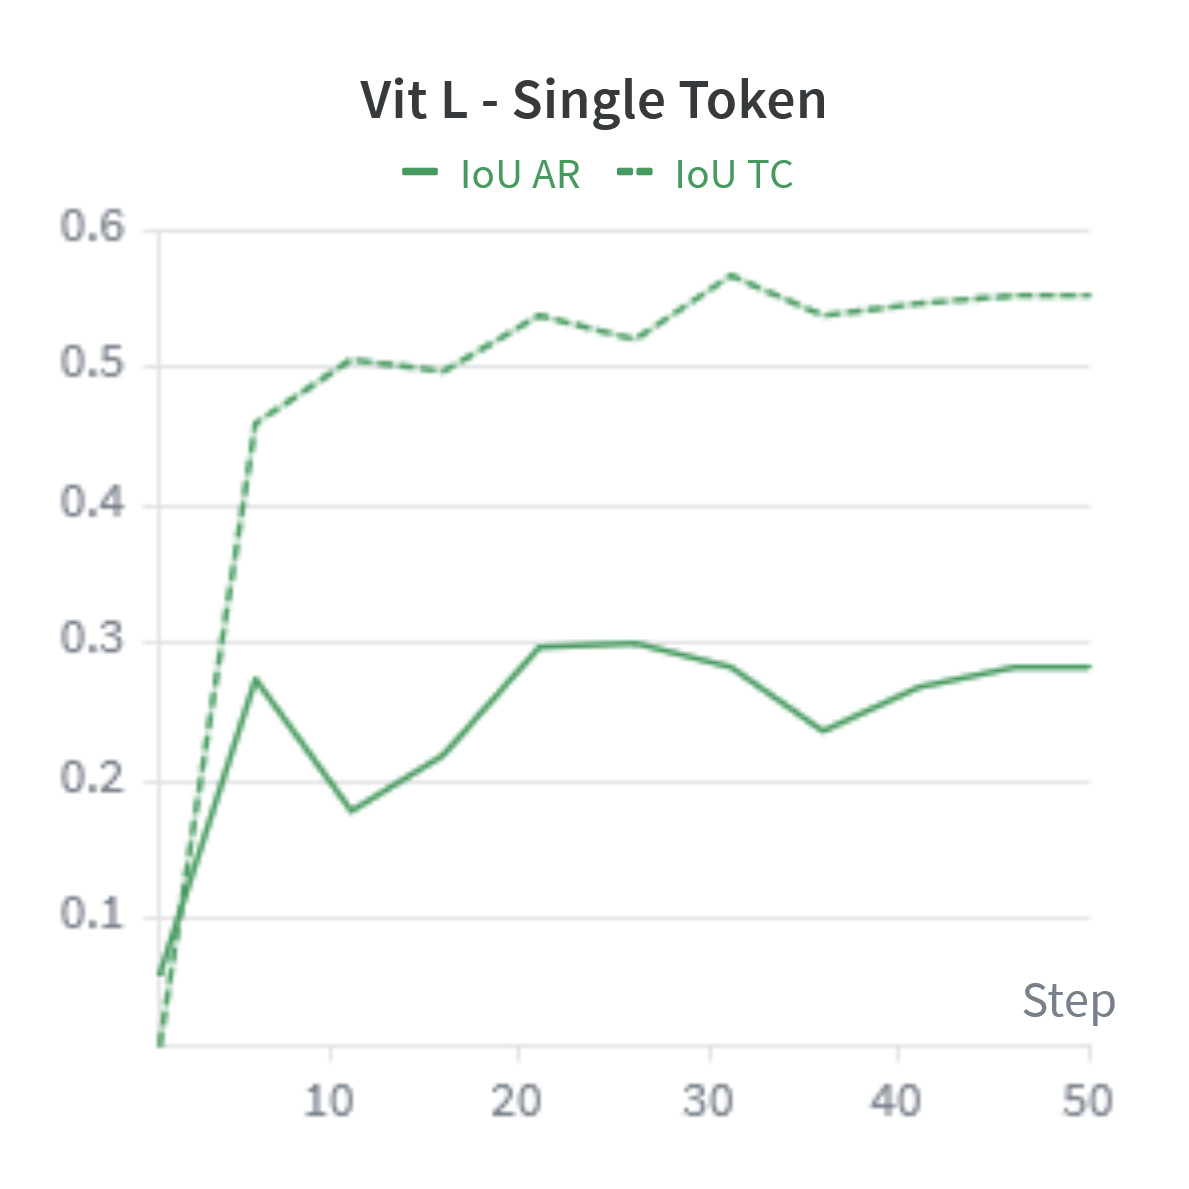
\includegraphics[width=\textwidth]{graphics/result/vitlsingletoken.png}
        % \caption{Vit L}
    \end{minipage}
    \caption{Validation IOU of TCs and ARs curves for SAM with single Token}
    \label{fig:iou_single_token}
\end{figure}




\subsubsection{SAM with Infused Specialized Token}

The training results indicate a positive correlation between the percentage of 
trainable parameters and model performance. As shown in Table 
\ref{tab:infused_token_params}, allocating a higher percentage of trainable 
weights enables the model to capture more complex features, though it increases 
computational demand. For instance, the vit\_l backbone with a 0.75 ratio 
utilizes 4.09\% of the total model (13.33M parameters) and requires 3.42 hours 
to achieve its peak performance. In contrast, the vit\_b backbone at a 0.50 
ratio remains more efficient, utilizing 4.46\% of its architecture (4.38M 
parameters) within 2.15 hours.

\begin{table}[h]
\centering
\begin{tabular}{lccc}
\hline
Backbone & MLP Ratio & IOU ARs & IOU TCs \\
\hline
vit\_l & 0.75 & 0.2426 & 0.5058 \\
vit\_b & 0.75 & 0.2810 & 0.5102 \\
vit\_l & 0.50 & 0.2787 & 0.2973 \\
vit\_b & 0.50 & 0.2867 & 0.5003 \\
\hline
\end{tabular}
\caption{Performance Comparison for Infused Token SAM}
\label{tab:infused_token_perf}
\end{table}

\begin{table}[h]
\centering
\begin{tabular}{lccccccc}
\hline
Backbone & MLP Ratio & Decoder & Encoder & Train & Total & \% Train & Time (h) \\
\hline
vit\_l & 0.75 & 1.47M & 11.86M & 13.33M & 325.68M & 4.09\% & 3.42 \\
vit\_b & 0.75 & 1.21M & 4.74M & 5.95M & 99.69M & 5.97\% & 2.10 \\
vit\_l & 0.50 & 1.47M & 7.92M & 9.39M & 321.74M & 2.92\% & 2.36 \\
vit\_b & 0.50 & 1.21M & 3.17M & 4.38M & 98.12M & 4.46\% & 2.15 \\
\hline
\end{tabular}
\caption{Detailed Parameter Breakdown and Training Duration for Infused Token SAM}
\label{tab:infused_token_params}
\end{table}

Despite the specialization of tokens, the model continues to struggle with catastrophic forgetting, as optimization for large scale ARs structures appears to overwrite the representations required for TCs. This task interference is likely exacerbated by the token integration mechanism; because the tokens are combined via element wise addition and divided by two, the resulting averaging effect may dilute specialized signals and hinder the maintenance of distinct representational boundaries. Consequently, while the larger vit\_l backbone provides increased capacity, the inherent token blending and task interference prevent a stable multi objective balance, leading to the observed decline in TCs performance as the model converges on ARs.


\subsubsection{SAM with Concatenated Specialized Token}
